\subsection{Quantifying stochasticity}
\label{app:seed-variation}

\begin{figure}[b!]
    \centering
    \begin{subfigure}[b]{0.47\textwidth}
        \centering
        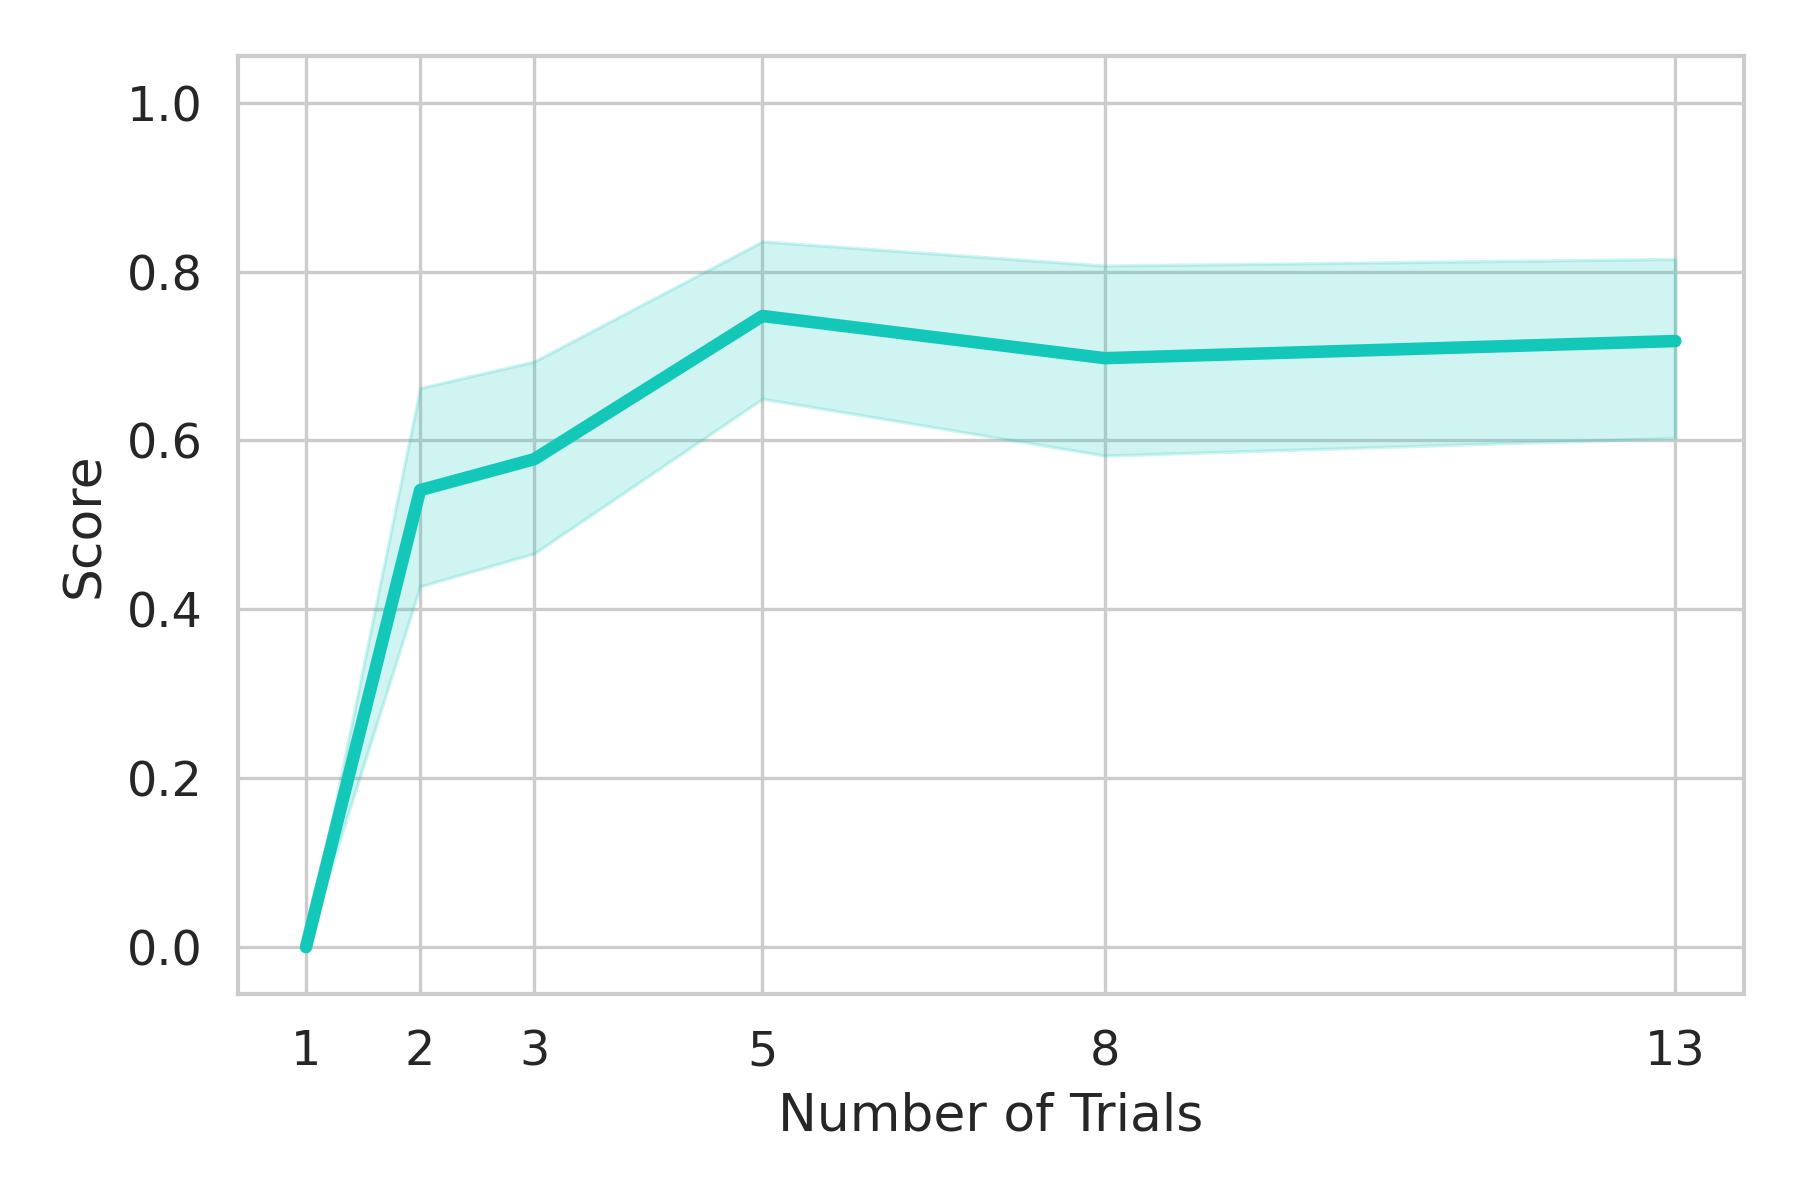
\includegraphics[width=\linewidth]{figures/task-variance.png}
        \vskip -3pt \caption{}
        \label{fig:task-variance}
    \end{subfigure}
    \begin{subfigure}[b]{0.47\textwidth}
        \centering
        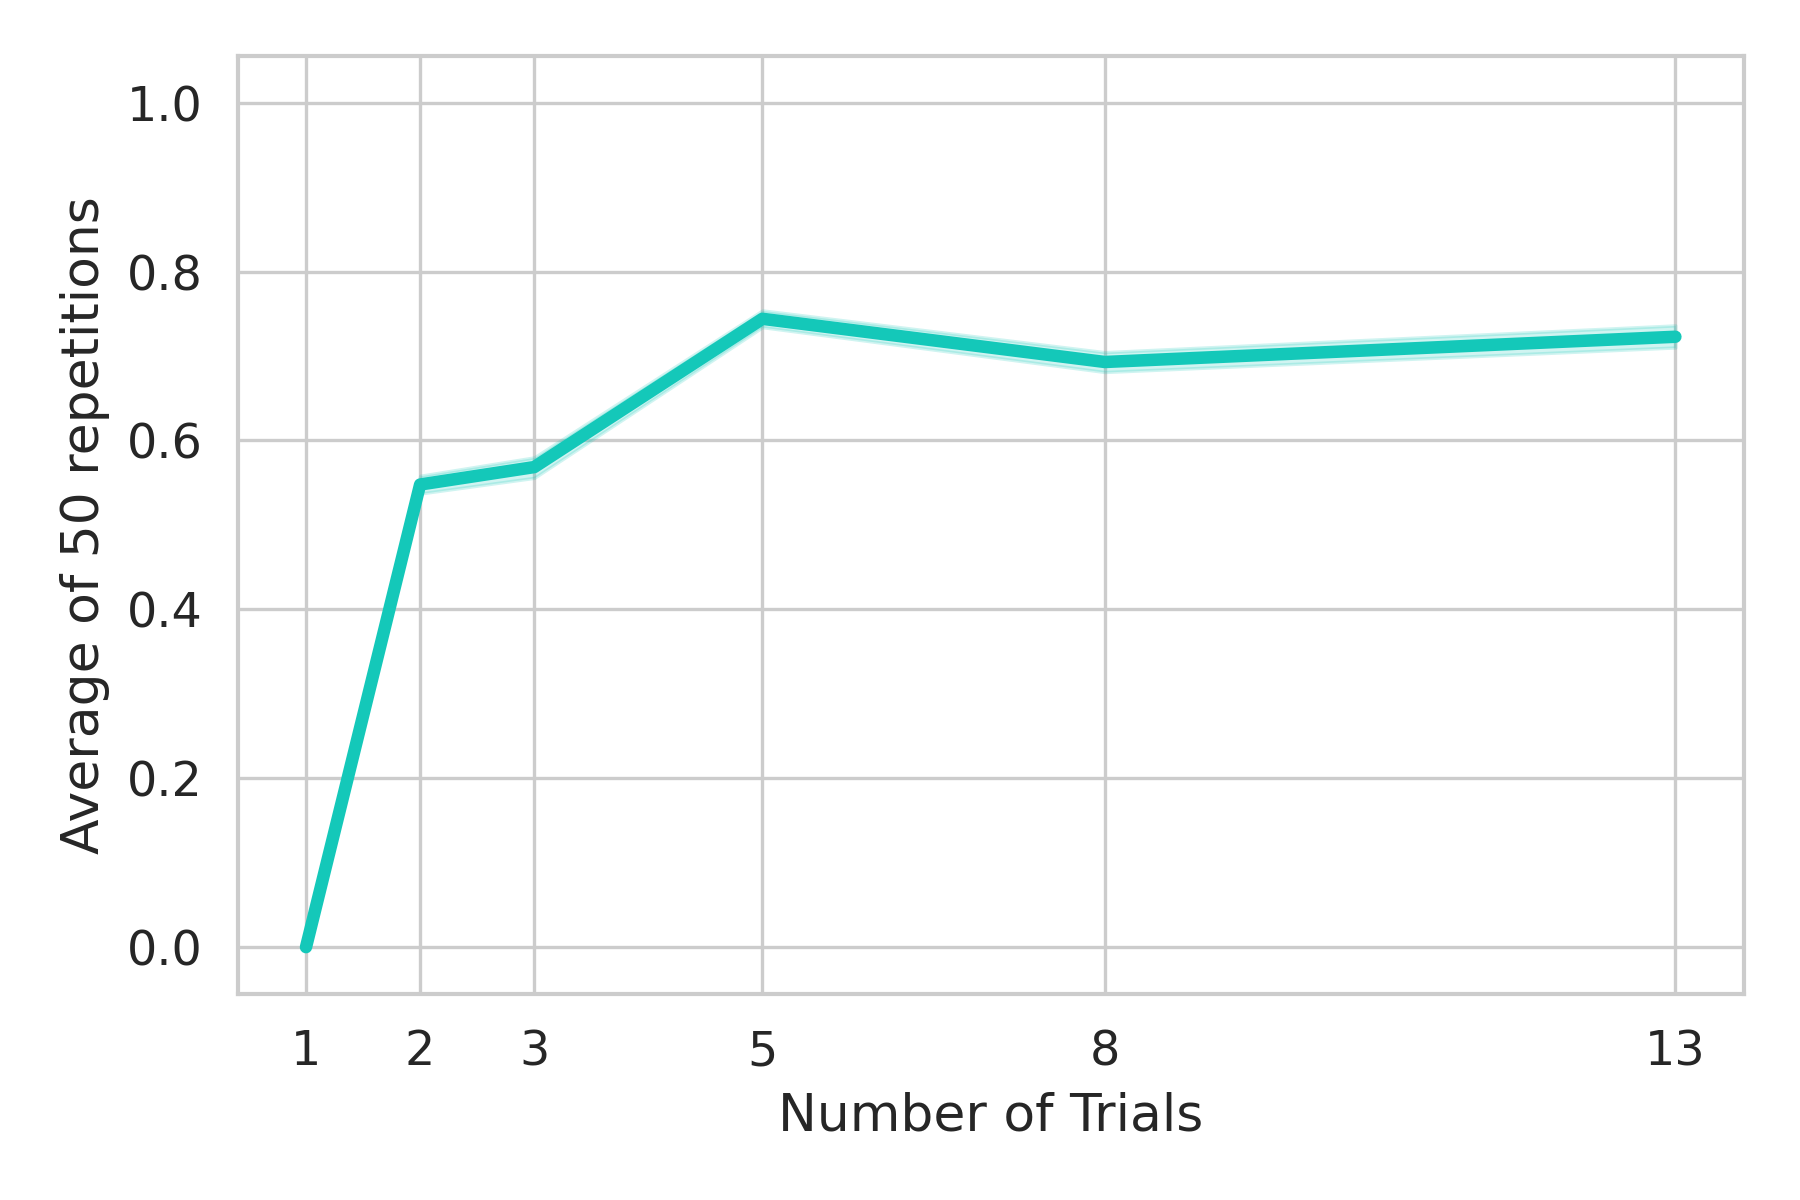
\includegraphics[width=\linewidth]{figures/task-variance-repetitions.png}
        \vskip -3pt \caption{}
        \label{fig:task-variance-repetitions}
    \end{subfigure}

    \caption{
        \textbf{(a)} Mean single-repetition score and 95\% confidence intervals over 50 samples.
        \textbf{(b)} Mean of the aggregated 50-repetition score and 95\% confidence intervals over 50 samples.}
\end{figure}

\paragraph{Task variation.} Figure \ref{fig:task-variance} shows that there is fairly high variance in the score obtained by a single agent over 50 repetitions of a single task. This is due to random spawn rotations of the avatar following every environment reset and stochasticity in the agent's policy. To address this we run 50 repetitions of every (task, $k$) combination and average the score over these repetitions. This reduces the standard deviation to that shown in Figure \ref{fig:task-variance-repetitions}. Here, the standard deviation of the mean task score reduced from a maximum of 0.43 with 1 repetition, to a maximum of 0.06 with 50 repetitions.

\begin{figure}[htb]
    \centering
    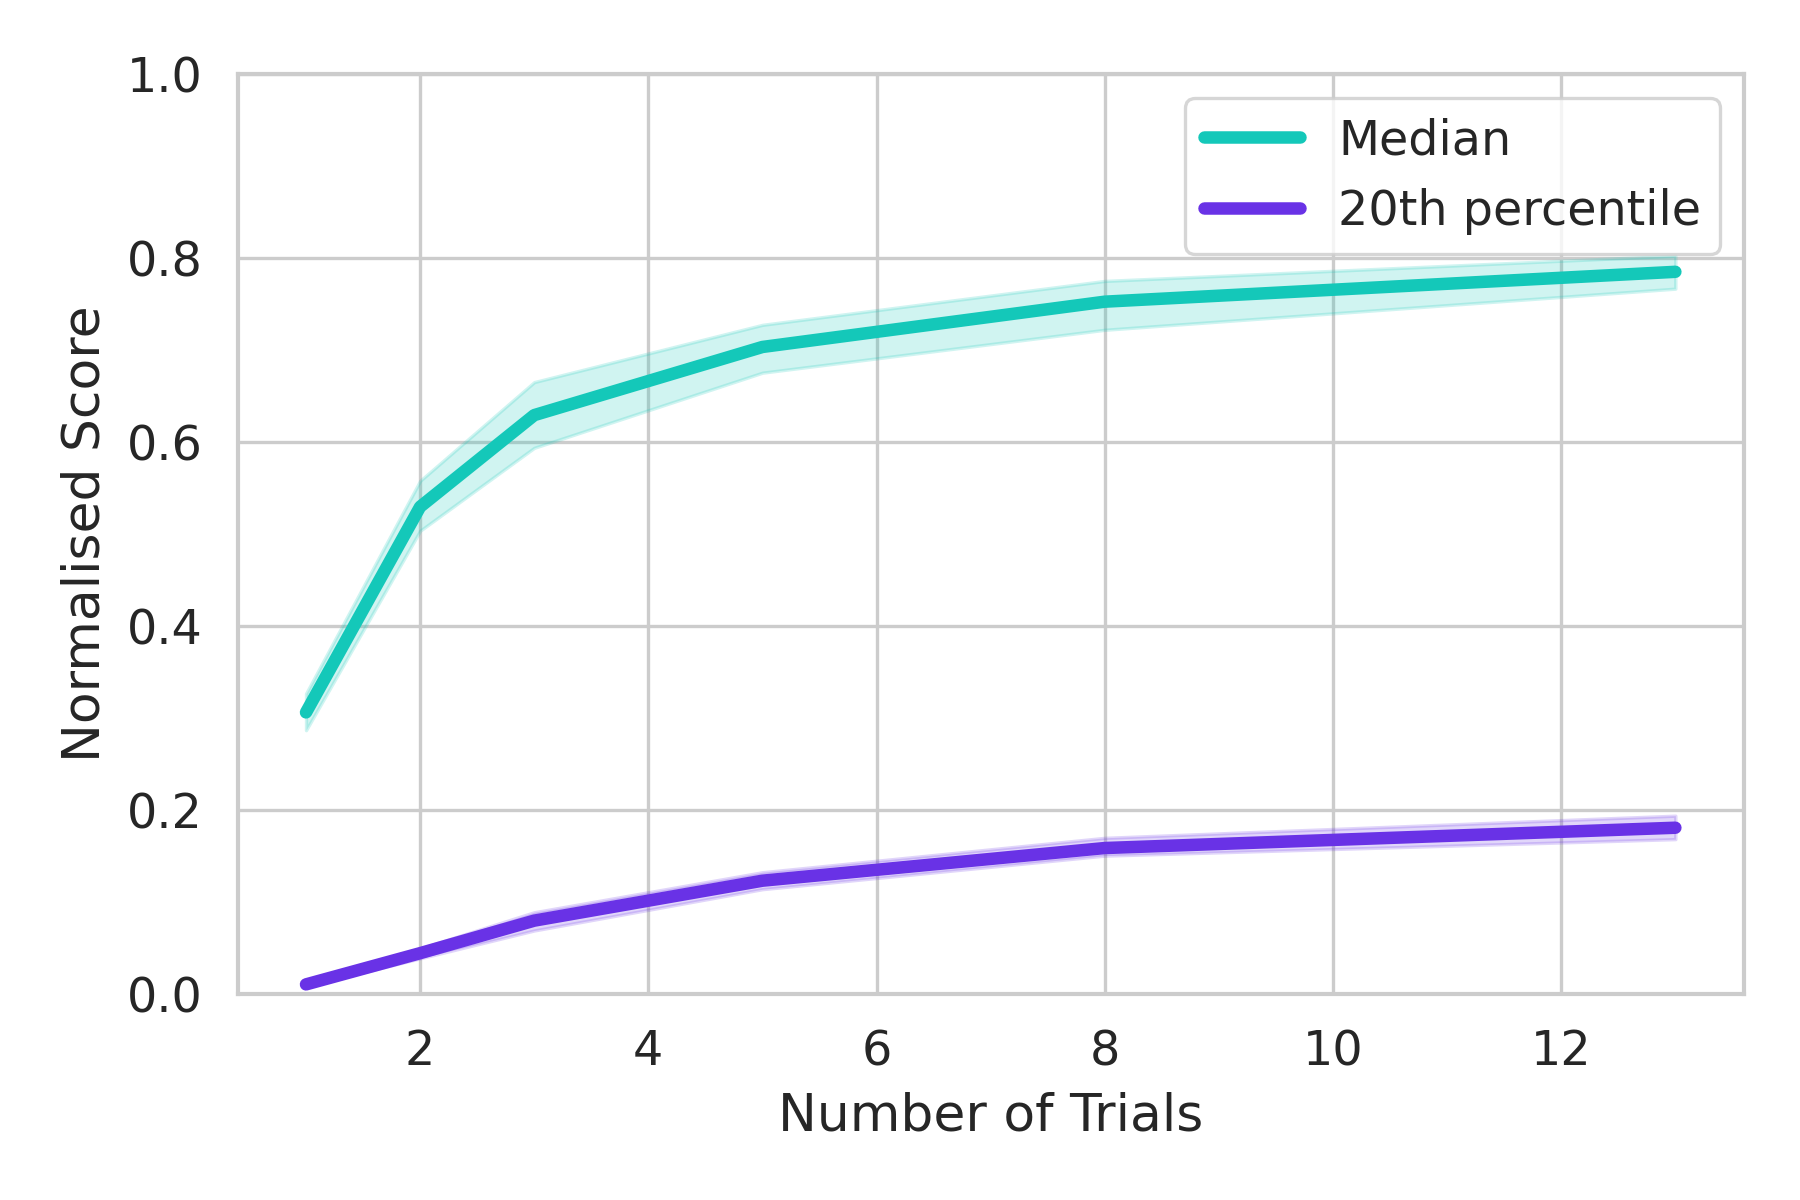
\includegraphics[width=0.5\linewidth]{figures/seed-variance.png}
    \caption{95\% bootstrap confidence intervals around the median and 20th percentile over our test set of 5 agents trained with different initialisation seeds. The maximum observed standard deviation was 0.04 around the median and 0.02 around the 20th percentile.}
    \label{fig:seed-variance}
\end{figure}

\paragraph{Agent initialisation variation.} After accounting for task variation, Figure \ref{fig:seed-variance} shows the variance due to agent initialisation seed during training. We plot the score as a function of $k$ on our test set for the 76M total parameter version of AdA with 5 different initialisation seeds. The maximum standard deviation observed for any number of trials in the median was 0.04 and for the 20\textsuperscript{th} percentile was 0.02. This low initialisation seed variance led us to run our ablations with one initialisation seed to save on compute. We note that the results shown in our ablation section have significantly larger than one standard deviation differences. 